\documentclass[main.tex]{subfiles}

\providecommand{\Par}{\operatorname{Parent}}
\newcommand{\LA}{\operatorname{LA}}
\newcommand{\Dep}{\operatorname{D}}
\newcommand{\LCA}{\operatorname{LCA}}
\newcommand{\argmax}{\operatorname{argmax}}

\begin{document}

\chapter{Ancestrais em árvores} \label{cap:ancestrais}

\section{Introdução}

Seja~$T \coloneqq (V, E)$ um grafo. Dizemos que~$T$ é uma árvore se é acíclico e conexo. Nesse caso, entre cada par de vértices de~$T$ existe exatamente um caminho. Uma árvore é enraizada quando fixamos algum vértice~${r \in V}$, chamado de raiz.

Para propósitos de implementação e sem perda de generalidade, supomos que~$V = \{1, 2, \ldots, |V|\}$.
Para cada vértice~${u \in V}$, os \deff{ancestrais} de~$u$ são os vértices no (único) caminho de~$u$ até~$r$. O~\mbox{$(i-1)$-ésimo} ancestral de~$u$ é o~$i$-ésimo vértice nesse caminho. Em particular,~$u$ é o $0$-ésimo ancestral de~$u$. Dizemos que o primeiro ancestral de~$u$, se~$u \neq r$, é o \deff{pai} de~$u$. Definimos a função~${\Par: V \rightarrow V}$ tal que~$\Par(u)$ é o pai do vértice~$u$, para todo~$u \in V \setminus \{r\}$; para o vértice~$r$, pode-se considerar que~$\Par(r) = r$. A~\deff{profundidade} de um vértice~$u$ é denotada por~$\Dep(u)$ e é o número de arestas no caminho de~$u$ até~$r$.

O problema do Ancestral de Nível (no inglês, \textit{Level Ancestor}, abreviado LA), é o problema de encontrar, dados~$u \in V$ e~$k \in \mathbb{N}$ tal que~$k \leq \Dep(u)$, o~$k$-ésimo ancestral de~$u$, ou seja, o problema de avaliar a função
$$\LA(k, u) \coloneqq \Par^k(u). $$

O problema do Primeiro Ancestral Comum (no inglês, \textit{Lowest Common Ancestor}, abreviado LCA), é o problema de encontrar, dados~$u, v \in V$, o vértice~$w$ de maior profundidade que é ancestral de ambos~$u$ e~$v$, ou seja, o problema de avaliar a função
$$\LCA(u, v) \coloneqq \argmax\{\Dep(w) : w \in V,\ w \text{ é ancestral de $u$ e $v$}\}. $$

\section{Potências de funções} \label{sec:potfunc}

Vamos considerar o problema, um pouco mais genérico, de, dada uma função~$f : [n] \rightarrow [n]$, que pode ser dada por um vetor de tamanho~$n$, por exemplo, construir um algoritmo que, após possivelmente algum pré-processamento sobre o vetor~$f$, responda consultas do tipo: dados~$i \in [n]$ e~$k \in [m] \cup \{0\}$, determinar~$f^k(i)$ de forma eficiente. Se o tempo de processamento é~$\Oh(p(n, m))$ e o tempo para responder cada consulta é~$\Oh(q(n, m))$, dizemos que a complexidade da solução é~$\angles{\Oh(p(n, m)), \Oh(q(n, m))}$.

\subsection{Soluções simples} \label{subsec:anc_sol_simples}

Uma solução simples é não fazer nenhum pré-processamento e sempre realizar as~$k$ iterações para determinar~$f^k(i)$. Esta solução tem complexidade~$\angles{\Oh(1),\Oh(m)}$. Outra solução simples é armazenar a resposta para todas as consultas possíveis em uma matriz~$M$ tal que~$M[k][i] = f^k(i)$ para todo~$i \in [n]$ e~$k \in [m] \cup \{0\}$. Esta matriz pode ser preenchida usando programação dinâmica em tempo~$\Oh(nm)$, já que sabemos que, se~$k > 0$, então~$f^k(i) = f(f^{k-1}(i))$, ou seja,
$$M[k][i] = \left\{
	\begin{array}{ll}
		f(M[k - 1][i]) & \text{ se $k > 0$} \\
		i & \text{ se $k = 0$,}
	\end{array}
	\right.
$$
ou seja, podemos preencher~$M$ iterando pelos seus índices em ordem não decrescente de~$k$. Esta solução tem complexidade~$\angles{\Oh(nm), \Oh(1)}$.

\subsection{Potências de dois} \label{subsec:pot2}

As soluções apresentadas funcionam da seguinte maneira: escolhe-se uma base~$(a_1, \ldots, a_x)$ tal que todo número entre~0 e~$m$ pode ser escrito como soma de zero ou mais destes números, e calcula-se (durante o pré-processamento)~$f^{a_j}(i)$ para todo~$i \in [n]$ e~$j \in [x]$. Dado um número~$k$, escreve-se este como~$k = a_{b_1} + a_{b_2} + \cdots + a_{b_y}$, e após isso calcula-se
$$f^k(i) = f^{a_{b_1}}(f^{a_{b_2}}(\cdots(f^{a_{b_y}}(i))\cdots)).$$
No primeiro exemplo da Subseção~\ref{subsec:anc_sol_simples} escolhemos como base apenas~$(1)$, e o tempo de consulta foi grande, enquanto no segundo exemplo escolhemos~$(1, \ldots, m)$, e o tempo de pré-processamento foi grande.

Escolhendo a base de forma mais inteligente, é possível melhorar a complexidade. Cada número tem uma decomposição (única) em somas de potências de dois distintas (correspondente à sua representação binária), e existem apenas~$\floor{\lg m}$ potências de~2 entre~1 e~$m$. Portanto, podemos escolher a base~${(1, 2, 4, \ldots, 2^{\floor{\lg m}})}$. Para fazer o pré-processamento, utilizaremos programação dinâmica preenchendo uma matriz~$M$ tal que~${M[k][i] \coloneqq f^{2^k}(i)}$ para todo~$i \in [n]$ e~$0 \leq k \leq \floor{\lg m}$. Sabemos que~$f^x(f^x(i)) = f^{2x}(i)$, logo temos
$$M[k][i] = \left\{
	\begin{array}{ll}
		M[k-1][M[k - 1][i]] & \text{ se $k > 0$} \\
		f(i) & \text{ se $k = 0$,}
	\end{array}
	\right.
$$
e também podemos preencher~$M$ iterando pelos seus índices em ordem não decrescente de~$k$.

\begin{theorem} \label{thm:pot2}
	Todo número positivo tem uma única decomposição em soma de potências de dois distintas.
\end{theorem}
\begin{proof}
	A prova é por indução. É óbvio que~1 tem uma única decomposição em soma de potências de dois.

	Seja~$k > 1$ um inteiro e seja~$2^x$ a maior potência de dois menor ou igual a~$k$. Note que~$k - 2^x < 2^x$ (caso contrário~$2^{x+1} \leq k$), então pela hipótese de indução~$k - 2^x$ tem uma decomposição em potências de dois distintas, e nenhuma destas potências é~$2^x$, logo podemos adicionar esta potência à representação. Isto prova a existência. A unicidade segue de que a representação de~$k - 2^x$ é única pela hipótese de indução e, como~$\sum\limits_{0 \leq y < x}{2^{y}} = 2^x - 1 < 2^x$, temos que qualquer decomposição de~$k$ deve conter~$2^x$.
\end{proof}

A prova acima nos dá um algoritmo para encontrar uma decomposição em potências de dois de~$k$: basta encontrar a maior potência de dois menor ou igual a~$k$ e subtraí-la de~$k$, e repetir este procedimento até~$k$ se tornar~0.

\begin{algorithm}
	\caption{Solução para potência de função.} \label{lst:potfunclg}
\begin{algorithmic}[1]
	\LineComment{Cria a matriz~$M$ a partir de~$f$.}
	\Function{Preprocessing}{$f, n, m$}
		\For{$i = 1 \To n$}
			\State $M[0][i] = f(i)$
		\EndFor
		\For{$k = 1 \To \floor{\lg m}$}
			\For{$i = 1 \To n$}
				\State $M[k][i] = M[k - 1][M[k - 1][i]]$
			\EndFor
		\EndFor
	\EndFunction

	\LineComment{Devolve~$f^k(i)$; deve ser chamada após~\textsc{Preprocessing}.}
	\Function{Query}{$k, i$} \Comment{$k \leq m$ e $i \leq n$}
		\For{$x = \floor{\lg{m}} \DownTo 0$}
			\If{$2^x \leq k$}
				\State $k = k - 2^x$
				\State $i = M[x][i]$
			\EndIf
		\EndFor
		\State \Return $i$
	\EndFunction
\end{algorithmic}
\end{algorithm}

O Código~\ref{lst:potfunclg} mostra a solução discutida, que tem complexidade~$\angles{\Oh(n\lg m), \Oh(\lg m)}$ e consome espaço~$\Oh(n \lg m)$. Note que é fácil implementar~\Call{Query}{$k, i$} de forma que esta consuma tempo~$\Oh(\lg k)$; basta, no laço, o valor de~$x$ começar com~$\floor{\lg k}$.

\section{Ancestral de nível online para árvores}

Como~$\Par$ é uma função de~$V$ em~$V$, é possível utilizar os algoritmos discutidos na Seção~\ref{sec:potfunc} para avaliar a função~$\LA$. Note que, para cada~$u \in V$, precisamos apenas calcular~$\Par^k(u)$ para~$k < \Dep(u)$, logo usamos~$n = m = |V|$. Estes algoritmos, porém, supõem que a função é conhecida de antemão, para realizar o pré-processamento, ou seja, a função~$\Par$ deve ser totalmente conhecida de antemão (e por conseguinte a árvore).

\newcommand{\jmp}{\mathit{jump}}
Na Subseção~\ref{subsec:pot2}, vimos que~$M[k][u] = M[k-1][M[k-1][u]]$ pode ser calculada usando programação dinâmica pois depende de índices menores da primeira coordenada. No caso de árvores, porém, sabemos que~$f^{2^{k-1}}(u)$ é um ancestral de~$u$, logo para calcular os valores~$M[k][u]$ para todo~${0 \leq k < \floor{\lg \Dep(u)}}$ basta que os valores de~$M$ já estejam calculados para todos os ancestrais de~$u$, e então calculamos~$M[k][u]$ em ordem crescente de~$k$ (já que~$M[k][u]$ depende de~$M[k-1][u]$ além de seus ancestrais).

Por esse motivo, o algoritmo pode ser implementado de forma online, com novas folhas podendo ser adicionadas à árvore. Para melhorar a notação neste caso, usamos em cada nó um vetor~$\jmp$ com os valores de~$M$, ou seja,~${u.\jmp[k] = M[k][u] = \Par^{2^k}(u)}$. Assim que uma folha~$u$ for adicionada, podemos calcular os valores de~$u.\jmp$, em tempo e espaço~${\Oh(\floor{\lg \Dep(u)})}$. A consulta continua da mesma forma.

\begin{algorithm}
\caption{Solução para o problema do Ancestral de Nível.} \label{lst:lapot2}
\begin{algorithmic}[1]
	\LineComment{Adiciona a folha~$u$ à árvore.}
	\Function{\API{AddLeaf}}{$u$}
		\State $u.\jmp[0] = \Par(u)$
		\For{$k = 1 \To \floor{\lg \Dep(u)}$}
			\State $u.\jmp[k] = u.\jmp[k - 1].\jmp[k - 1]$
		\EndFor
	\EndFunction

	\LineComment{Devolve~$\LA(k, u)$; deve ser chamada após~\funcAPI{AddLeaf}{u}.}
	\Function{\API{LevelAncestor}}{$k, u$}
		\For{$x = \floor{\lg{k}} \DownTo 0$}
			\If{$2^x \leq k$}
				\State $k = k - 2^x$
				\State $u = u.\jmp[x]$
			\EndIf
		\EndFor
		\State \Return $u$
	\EndFunction
\end{algorithmic}
\end{algorithm}

O Código~\ref{lst:lapot2} resolve o problema do Ancestral de Nível online, quando se pode adicionar folhas à árvore. A operação~$\funcAPI{AddLeaf}{u}$ consome tempo~$\Oh(\lg \Dep(u))$ e a operação~$\funcAPI{LevelAncestor}{k, u}$ consome tempo~$\Oh(\lg k) = \Oh(\lg \Dep(u))$. Note que cada nó~$u$ deve armazenar um vetor de tamanho~$\floor{\lg \Dep(u)}$. Na literatura, essa técnica é chamada de Sparse Table, já que ``armazenamos'' uma tabela de tamanho~$|V| \times |V|$ usando apenas espaço~$|V| \lg |V|$, ou~Jump Pointers, neste caso mais específico do Ancestral de Nível em árvores~\cite{BenderM-F2004}. A Figura~\ref{fig:treejmppot2} ilustra os jump pointers de uma árvore.

\begin{figure}[h]
\centering
	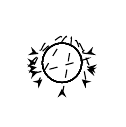
\begin{tikzpicture}[nodes={draw, circle, minimum size=5mm}, sibling distance=25pt, edge from parent/.append style={<-, shorten <= 2pt, shorten >= 2pt}, level distance=35pt]
	\Tree [.\node(v1){}; [.\node(v2){}; [.\node(v3){}; [.\node(v4){}; [.\node(v5){}; ] ] [.\node(v6){}; [.\node(v7){}; ] ] ] [.\node(v8){}; ] [.\node(v9){}; ] ] [.\node(v10){}; [.\node(v11){}; ] ] ]

		\tikzstyle{p2}=[->, shorten >= 2pt, shorten <= 2pt, dashed, >=stealth]
		\tikzstyle{p4}=[->, shorten >= 2pt, shorten <= 2pt, dotted, >=stealth]

		\draw[p2] (v3) edge[out=90,in=180] (v1);
		\draw[p2] (v4) edge[out=10,in=200] (v2);
		\draw[p2] (v5) edge[out=130,in=190] (v3);
		\draw[p4] (v5) edge[out=150,in=160] (v1);
		\draw[p2] (v8) edge[out=70,in=270] (v1);
		\draw[p2] (v9) edge[out=60,in=-40] (v1);
		\draw[p2] (v11) edge[out=30,in=20] (v1);
		\draw[p4] (v7) edge[out=0,in=-10] (v1);
		\draw[p2] (v6) edge[out=80,in=220] (v2);
		\draw[p2] (v7) edge[out=50,in=-15] (v3);
\end{tikzpicture}
	\caption{Exemplo de árvore com jump pointers. As arestas cheias são as arestas de pai~($\jmp[0]$), as arestas tracejadas pulam dois níveis~($\jmp[1]$), e as arestas pontilhadas pulam quatro níveis~($\jmp[2]$).} \label{fig:treejmppot2}
\end{figure}

\section{Cálculo do ancestral comum mais profundo} \label{sec:lca_pot2}

\newcommand{\kb}{k^\star}
Sejam~$u, v \in V$ e~$c \in V$ o ancestral comum mais profundo de~$u$ e~$v$. Vamos supor, sem perda de generalidade, que~${\Dep(v) \geq \Dep(u)}$. É óbvio que~${\Dep(c) \leq \Dep(u)}$, logo podemos ``nivelar'' os vértices~$u$ e~$v$, ou seja, trocar~$v$ por~${\LA(\Dep(v) - \Dep(u), v)}$.
Assim, podemos supor que~$\Dep(u) = \Dep(v)$ e, para encontrar o ancestral comum mais profundo de~$u$ e~$v$, devemos encontrar o menor~$\kb$ tal que~${\LA(\kb, u) = \LA(\kb, v)}$. Note que se~${k < \Dep(u) - 1}$ e~${\LA(k, u) = \LA(k, v)}$, então
$${\LA(k + 1, u) = \Par(\LA(k, u)) = \Par(\LA(k, v)) = \LA(k + 1, v).}$$
Isso permitirá a utilização dos Jump Pointers para determinar tal~$\kb$ mínimo.

Se~${x < \kb}$ então~${\LA(x, u) \neq \LA(x, v)}$, ou seja, temos uma forma de checar se~$x < \kb$ sem conhecer~$\kb$. Como, pela prova do Teorema~\ref{thm:pot2}, para decompor um número em soma de potências de dois distintas, basta determinar a maior potência de dois menor ou igual a esse número, adicioná-la à decomposição e repetir. Como temos jump pointers para as potências de dois para todos os nós, conseguimos determinar a decomposição em potências de dois distintas de~${\kb - 1}$ (já que conseguimos testar~${x \leq \kb - 1}$ e não~${x \leq \kb}$), e de forma similar à função~\API{LevelAncestor} do Código~\ref{lst:lapot2}, podemos determinar o~\mbox{$(\kb-1)$-ésimo} ancestral de~$u$ e~$v$ em tempo~$\Oh(\lg \Dep(u))$.

\begin{algorithm}
\caption{Primeiro Ancestral Comum usando Jump Pointers. \label{lst:lcapot2}}
\begin{algorithmic}[1]
	\Function{\API{LowestCommonAncestor}}{$u, v$}
		\If{$\Dep(u) > \Dep(v)$}
			\State $u, v = v, u$ \Comment{Garante que~$\Dep(u) \leq \Dep(v)$.}
		\EndIf
		\State $v = \funcAPI{LevelAncestor}{\Dep(v) - \Dep(u), v}$ \Comment{Nivela~$v$.}
		\If{$u = v$} \label{lst:lcapot2:if2}
			\State \Return $u$
		\EndIf
		\For{$i = \floor{\lg \Dep(u)} \DownTo 0$} \label{lst:lcapot2:for}
			\If{$u.\jmp[i] \neq v.\jmp[i]$} \label{lst:lcapot2:iffor}
				\State $u = u.\jmp[i]$
				\State $v = v.\jmp[i]$
			\EndIf
		\EndFor
		\LineComment{$u$ é agora o filho do LCA de~$u$ e~$v$.}
		\State \Return $\Par(u)$
	\EndFunction
\end{algorithmic}
\end{algorithm}

\begin{invar}
Ao início da iteração com valor~$i$ do~\keyword{for} da linha~\nref{lst:lcapot2:for} do Código~\ref{lst:lcapot2}, vale que~${0 < \Dep(u) - \Dep(c) \leq 2^{i+1}}$, onde~${c = \LCA(u, v)}$, e o valor de~$\LCA(u, v)$ não se altera ao final da iteração.
\end{invar}
\begin{proof}
	Para a base,~$i = \floor{\lg\Dep(u)}$ e
	$$\Dep(u) - \Dep(c) \leq \Dep(u) = 2^{\lg\Dep(u)} \leq 2^{\floor{\lg\Dep(u)}+1}.$$
	Além disso, se~$u = c$, então o~\keyword{if} da linha~\nref{lst:lcapot2:if2} é executado, logo~${\Dep(u) - \Dep(c) > 0}$.

	Suponha que o invariante vale ao início da iteração com valor~$i$, e provaremos que continua valendo ao começo da iteração com valor~$i - 1$. Seja~${d \coloneqq \Dep(u) - \Dep(c)}$. Sabemos então que~${0 < d \leq 2^{i+1}}$. Note que~${d \leq 2^i}$ se e somente se ${\LA(2^i, u) = \LA(2^i, v)}$, ou seja, o~\keyword{if} da linha~\nref{lst:lcapot2:iffor} é executado se e somente se~$d > 2^i$. Então
	\begin{itemize}
		\item se~$d \leq 2^i$, o invariante já vale para~$i-1$ e o~\keyword{if} não é executado;
		\item se~$d > 2^i$, o~\keyword{if} é executado, portanto trocamos~$u$ por~$\LA(2^i, u)$ e~$v$ por~$\LA(2^i, v)$. Seja~$d'$ o novo valor de~$\Dep(u) - \Dep(c)$. A profundidade de~$u$ e~$v$ diminui de~$2^i$, logo o valor de~$$d' = d - 2^i \leq 2^{i+1} - 2^i = 2^i.$$
		Como~$d > 2^i$, também temos que~${d' = d - 2^i > 0}$, e o invariante continua a valer.
	\end{itemize}
\end{proof}

Portanto, ao final da última iteração, o invariante vale para~$i = -1$, ou seja, vale que~${0 < \Dep(u) - \Dep(c) \leq 2^0 = 1}$, logo~$c$ é o pai de~$u$ e a função retorna o valor correto.

A Tabela~\ref{tab:la_pot2} mostra o consumo de tempo e espaço das implementações discutidas nesse capítulo.

\begin{table}[h] \centering
\begin{tabular}{|l|c|}
	\hline
	Função & Tempo/Espaço \\ \hline
	\funcAPI{AddLeaf}{u} & $\Oh(\lg n) / \Oh(\lg n)$ \\
	\funcAPI{LevelAncestor}{k, u} & $\Oh(\lg n) $ \\
	\funcAPI{LowestCommonAncestor}{u, v} & $\Oh(\lg n)$ \\ \hline
\end{tabular}
	\caption{Consumo de tempo e espaço da solução discutida, onde~$n$ é o tamanho da árvore.} \label{tab:la_pot2}
\end{table}

\end{document}
